\documentclass[compress]{beamer}
\usepackage{ifthen,verbatim}

\title{Misalignment studies with the official scenarios}
\author{Jim Pivarski, Alexei Safonov}
\institute{Texas A\&M University}
\date{30 November, 2007}

\newcommand{\isnote}{}
\xdefinecolor{lightyellow}{rgb}{1.,1.,0.25}
\xdefinecolor{darkblue}{rgb}{0.1,0.1,0.7}

%% Uncomment this to get annotations
%% \def\notes{\addtocounter{page}{-1}
%%            \renewcommand{\isnote}{*}
%% 	   \beamertemplateshadingbackground{lightyellow}{white}
%%            \begin{frame}
%%            \frametitle{Notes for the previous page (page \insertpagenumber)}
%%            \itemize}
%% \def\endnotes{\enditemize
%% 	      \end{frame}
%%               \beamertemplateshadingbackground{white}{white}
%%               \renewcommand{\isnote}{}}

%% Uncomment this to not get annotations
\def\notes{\comment}
\def\endnotes{\endcomment}

\setbeamertemplate{navigation symbols}{}
\setbeamertemplate{headline}{\includegraphics[height=1 cm]{../cmslogo} \hspace{0.1 cm} \includegraphics[height=1 cm]{../tamulogo} \hfill
\begin{minipage}{5.5 cm}
\vspace{-0.75 cm} \small
\begin{center}
\ifthenelse{\equal{\insertpagenumber}{1}}{}{\textcolor{blue}{\insertsection}}
\end{center}
\end{minipage} \hfill
\begin{minipage}{4.5 cm}
\vspace{-0.75 cm} \small
\begin{flushright}
\ifthenelse{\equal{\insertpagenumber}{1}}{}{Jim Pivarski \hspace{0.5 cm} \insertpagenumber\isnote/\pageref{numpages}}
\end{flushright}
\end{minipage}\mbox{\hspace{0.2 cm}}}

\begin{document}
\frame{\titlepage}

%% \begin{notes}
%% \item This is the annotated version of my talk.
%% \item If you want the version that I am presenting, download the one
%% labeled ``slides'' on Indico (or just ignore these yellow pages).
%% \item The annotated version is provided for extra detail and a written
%% record of comments that I intend to make orally.
%% \item Yellow notes refer to the content on the {\it previous} page.
%% \item All other slides are identical for the two versions.
%% \end{notes}

\section*{Misalignment studies}

\begin{frame}
\frametitle{Status of Alignment}
\begin{itemize}\setlength{\itemsep}{0.5 cm}
\item Alignment procedure: after discovering an error, we corrected
and re-tuned our procedure (last few weeks).  I am now setting it up
to re-do a full CSA07 exercise.

\item Quality of realistic procedure: slightly better than official
scenarios in $r\phi$, especially in wheel/disk placement.

\item Alignment studies with official scenarios: made all the relevant
plots, but discovered a mistake in my configuration.  Plots can be
recreated in a matter of hours.

\item Comparison with toy alignment: Ivan and I will talk offline?
\end{itemize}
\end{frame}

\begin{frame}
\frametitle{Alignment studies with official scenarios}
\begin{itemize}\setlength{\itemsep}{0.25 cm}
\item Using official $Z'_{SSM}$ and $Z'_\psi$ datasets (1--3.5 TeV) in 1\_6\_7
\item Full track reconstruction with each alignment configuration \\
(misalignment can cause tracks to lose hits or not be found)
\item 8 detector configurations:
\begin{center}
\begin{tabular}{c c}
tracker & muon system \\\hline
ideal & ideal \\
100~pb$^{-1}$ scenario & 100~pb$^{-1}$ scenario \\
10~pb$^{-1}$ scenario & 10~pb$^{-1}$ scenario \\
100~pb$^{-1}$ scenario & ideal \\
10~pb$^{-1}$ scenario & ideal \\
ideal & 100~pb$^{-1}$ scenario \\
ideal & 10~pb$^{-1}$ scenario \\
startup (laser alignment) & startup (10~pb$^{-1}$) \\
\end{tabular}
\end{center}
\end{itemize}
\end{frame}

\begin{frame}
\frametitle{The plots I'm about to show are place-holders}

I tracked a strange feature in the plots to a misconfiguration.  \\
\textcolor{darkblue}{Detective story in reverse order:}
\begin{itemize}\setlength{\itemsep}{0.25 cm}
\item To conserve disk space, I'm saving re-reconstructed events in
AlCaReco format (only saves tracks and hits) \\ Default cut is track $p_T$ $<$ 999~GeV

\item \begin{minipage}{0.45\linewidth}All samples cut off sharply at $\frac{1}{p_T} = 0.001$~GeV$^{-1}$\end{minipage} \hfill \begin{minipage}{0.5\linewidth}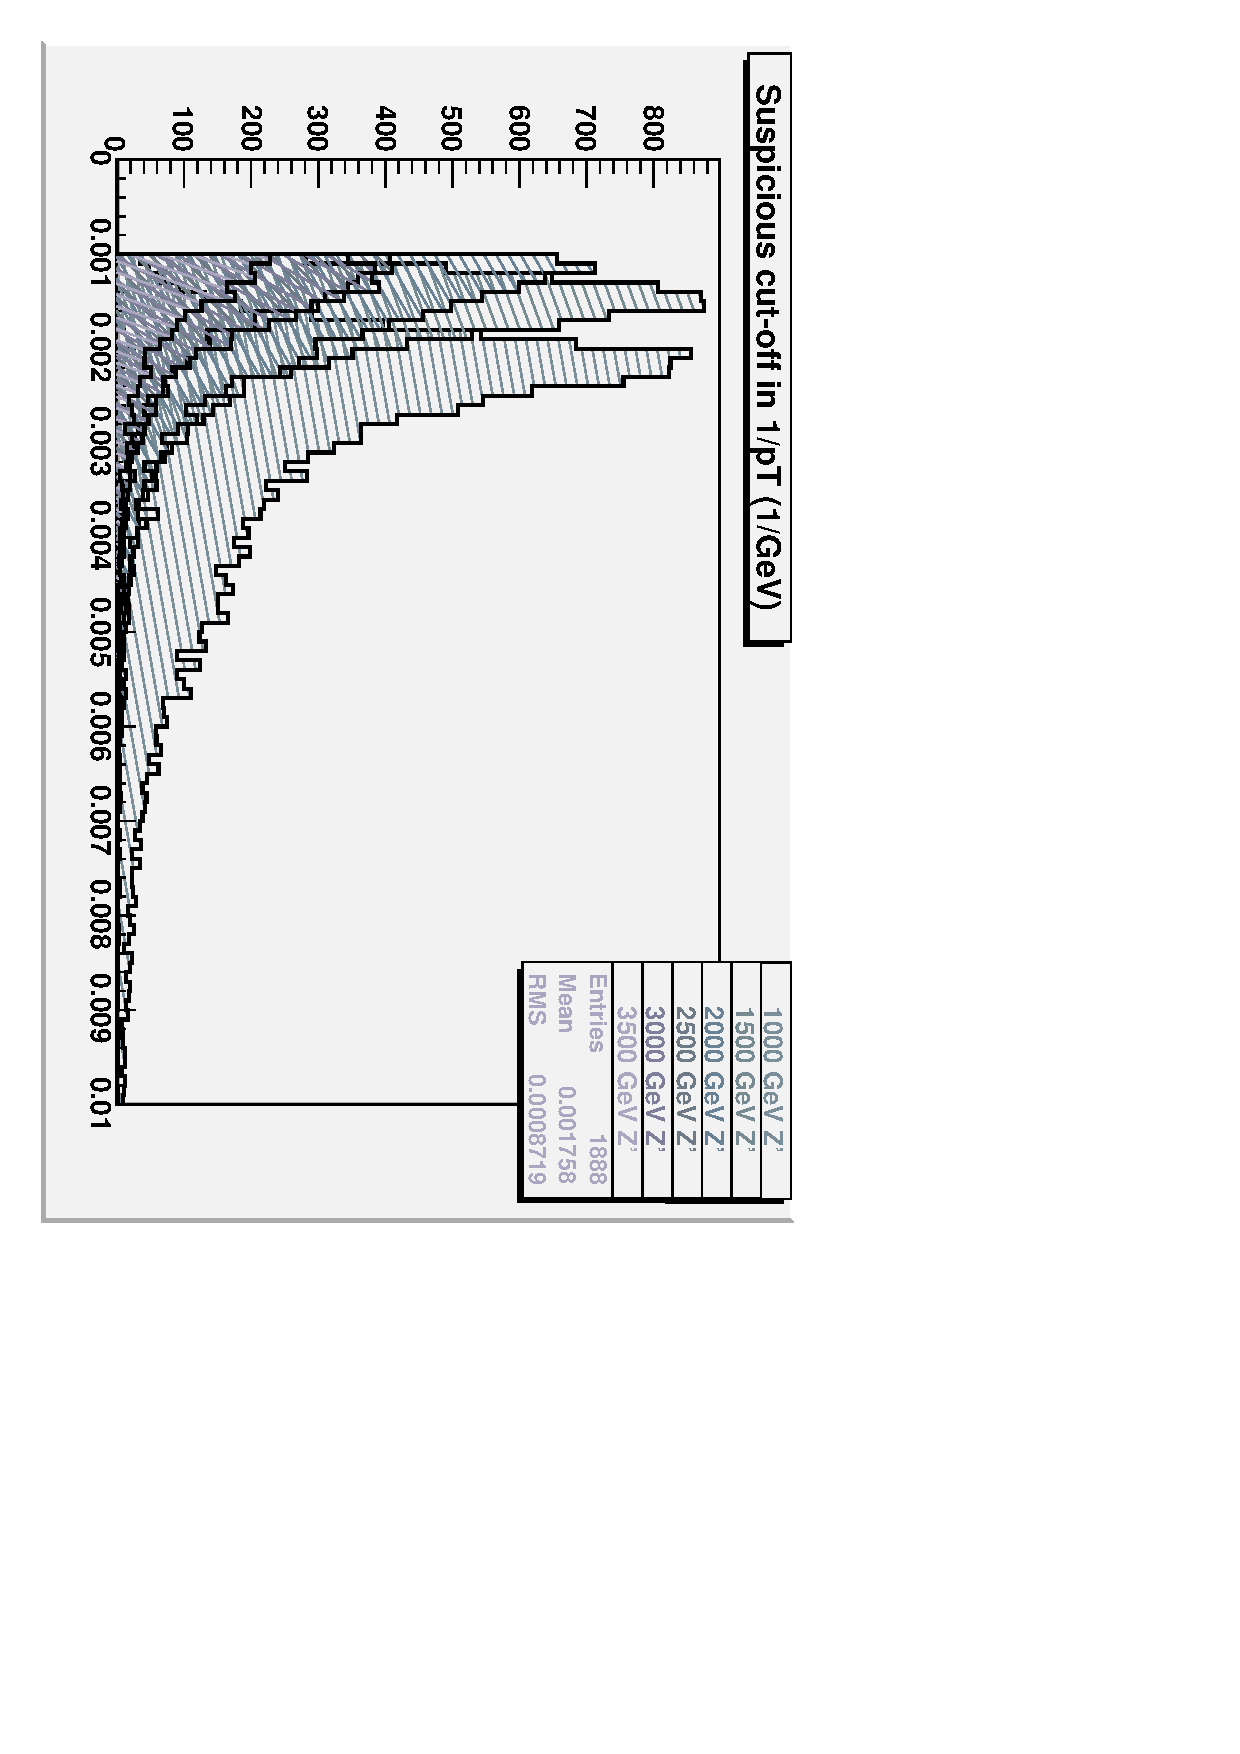
\includegraphics[height=\linewidth, angle=90]{suspicious.pdf}\end{minipage}

\item Causes a bias in track resolution near 1~TeV, a bias in dimuon masses above 2~TeV, and an inefficiency above 2~TeV
\end{itemize}
\end{frame}

\begin{frame}
\begin{center}
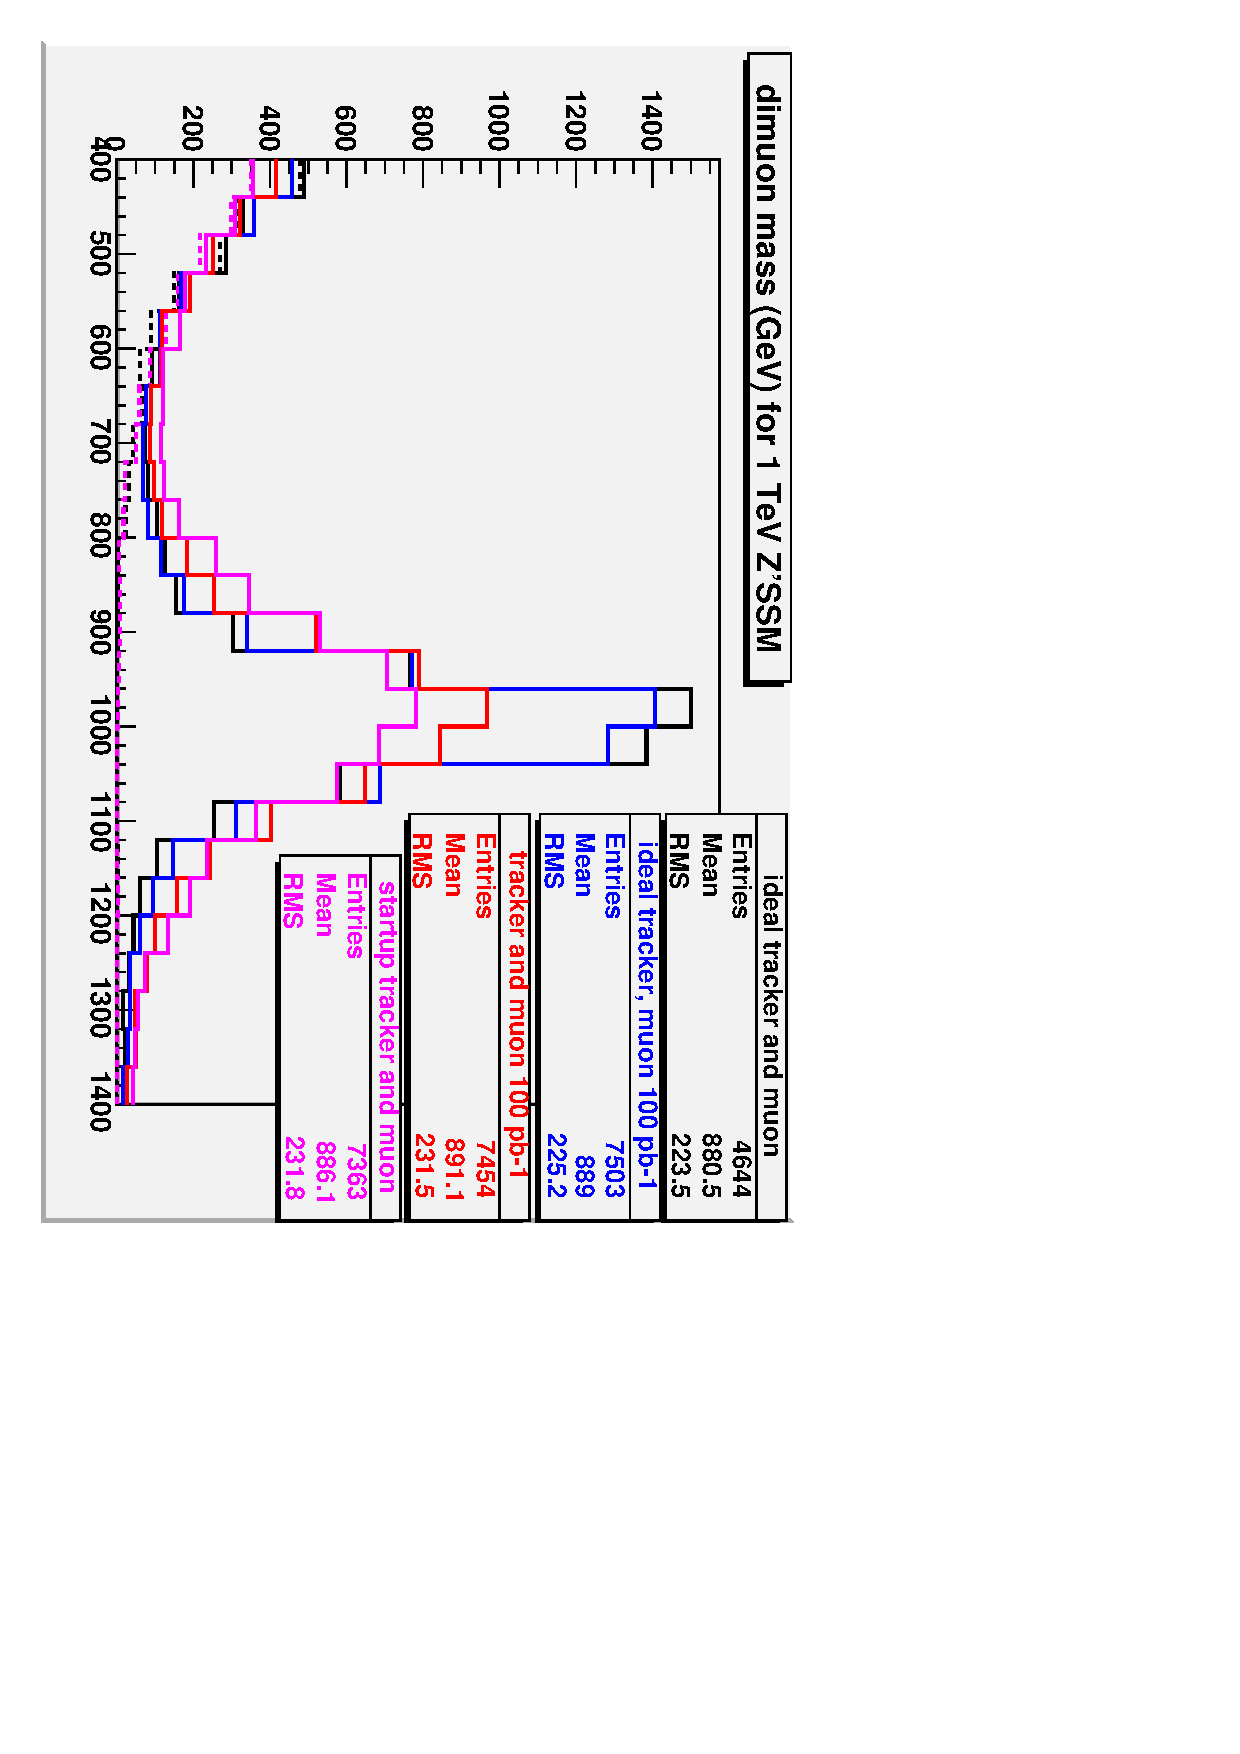
\includegraphics[height=0.9\linewidth, angle=90]{smear_1TeV.pdf}
\end{center}

\vspace{-0.25 cm}
\begin{itemize}
\item 1 TeV $Z'$ is minimally affected by track cut
\item Muon misalignment gets more interesting at higher energies
\item For resolution studies, we cut out Drell-Yan at generator level
\end{itemize}
\end{frame}

%% \begin{frame}
%% \begin{center}
%% 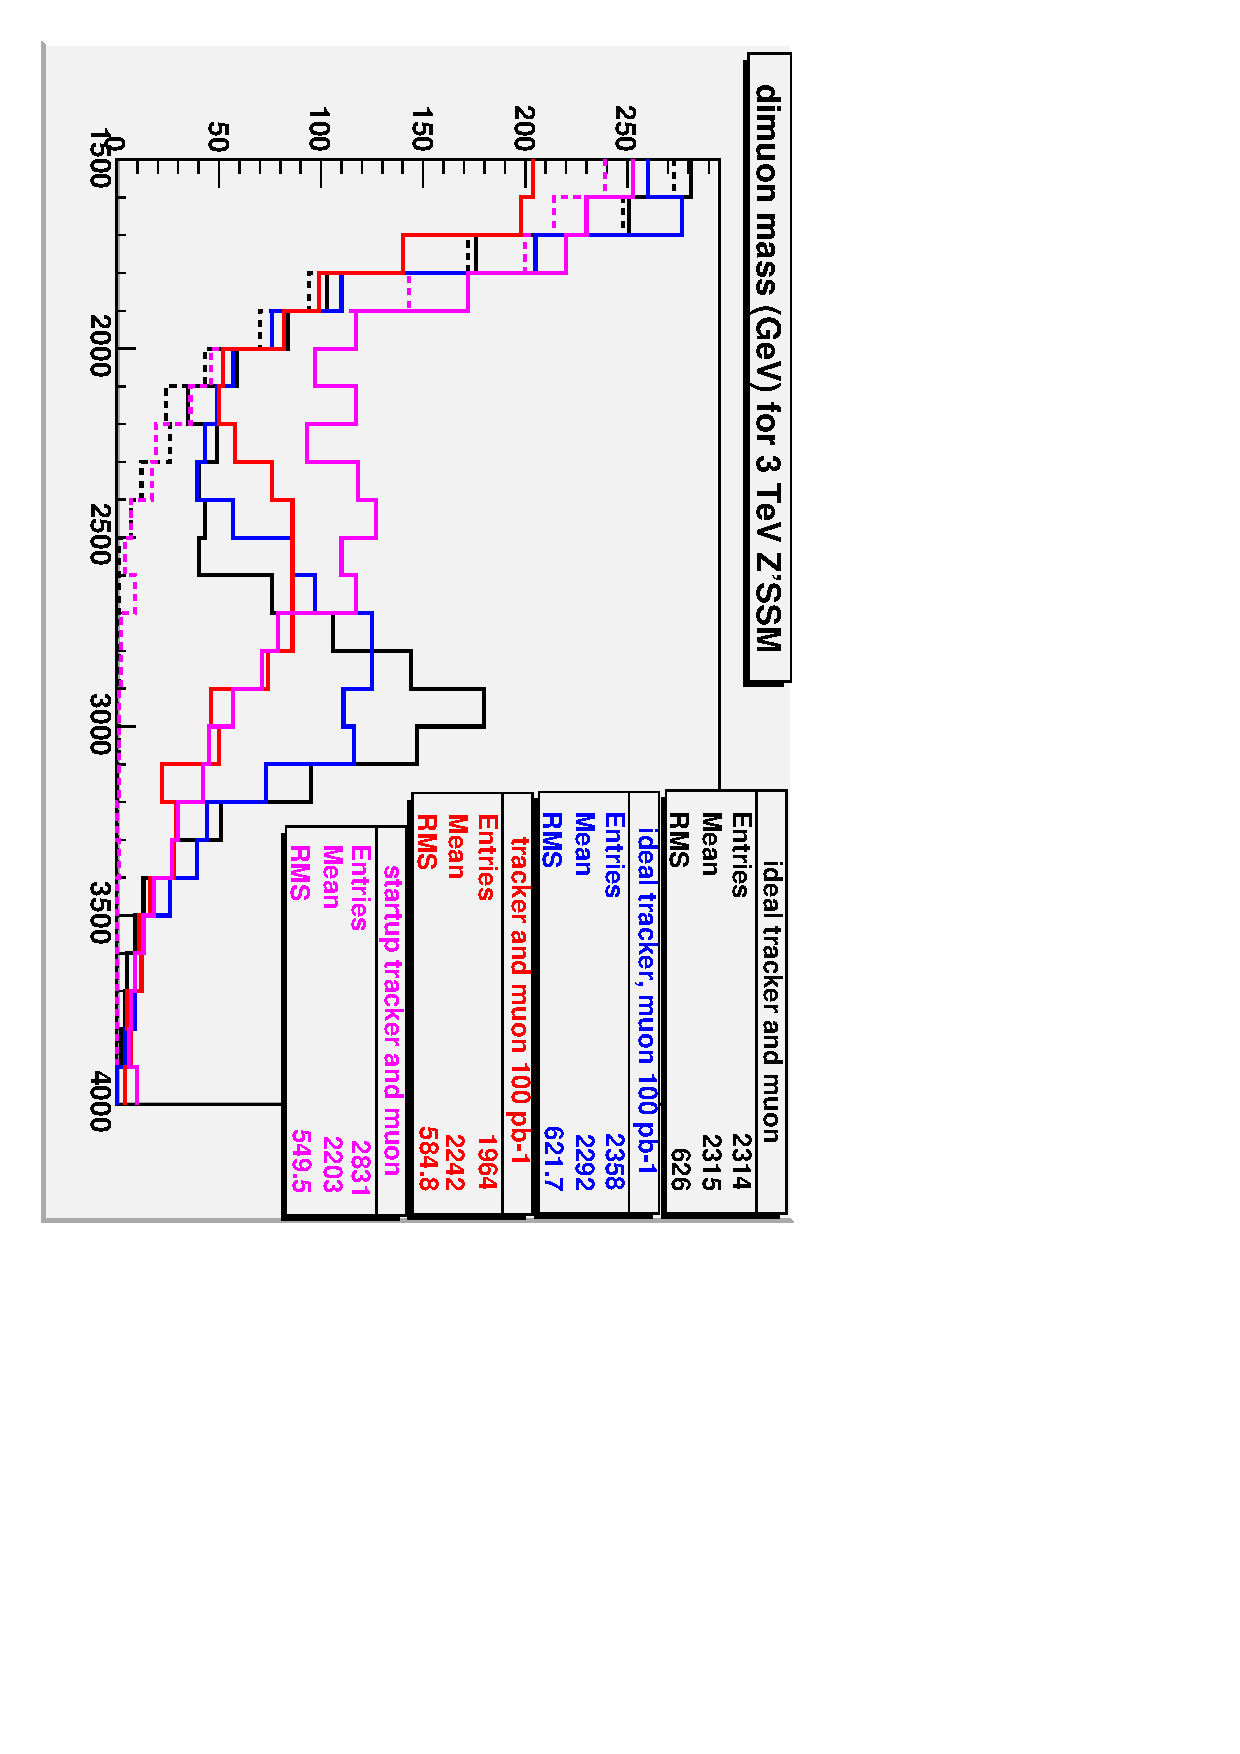
\includegraphics[height=0.9\linewidth, angle=90]{smear_3TeV.pdf}
%% \end{center}
%% \begin{itemize}
%% \item bias in 3 TeV $Z'$ is due to track cut (but how much?)
%% \end{itemize}
%% \end{frame}

\begin{frame}
\frametitle{Dimuon mass resolution}
\begin{itemize}
\item Resolution is width of \{reconstructed mass minus generated\}
\item Double-Gaussian fit for width (probably unnecessary w/o cut)
\item Expectations: increase with mass, \textcolor{blue}{ideal
tracker} better at low masses, \textcolor{red}{ideal muon} better at
high masses
\end{itemize}
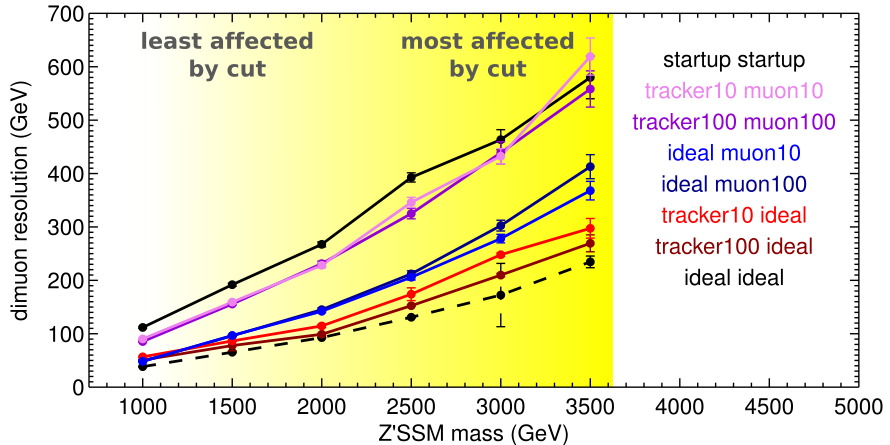
\includegraphics[width=\linewidth]{zssm_widths.png}
\end{frame}

\begin{frame}
\frametitle{Dimuon mass bias}
\begin{itemize}
\item Bias is centroid of \{reconstructed mass minus generated\}
\item May be entirely due to cut: wide distributions have most bias
\end{itemize}
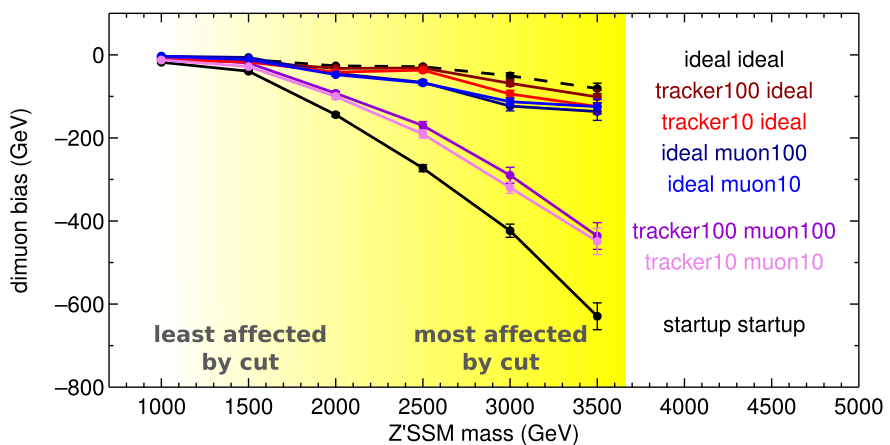
\includegraphics[width=\linewidth]{zssm_bias.png}
\end{frame}

\begin{frame}
\frametitle{Individual tracks}
\begin{itemize}
\item Resolution is width of $\displaystyle \frac{{p_T}^{\mbox{\scriptsize reco}} - {p_T}^{\mbox{\scriptsize gen}}}{{p_T}^{\mbox{\scriptsize gen}}}$ $=$ width of $\displaystyle \frac{{\kappa}^{\mbox{\scriptsize reco}} - {\kappa}^{\mbox{\scriptsize gen}}}{{\kappa}^{\mbox{\scriptsize gen}}}$
\item \textcolor{blue}{misaligned muon} matters above 400~GeV
\item \textcolor{red}{misaligned tracker} is fairly constant
\end{itemize}
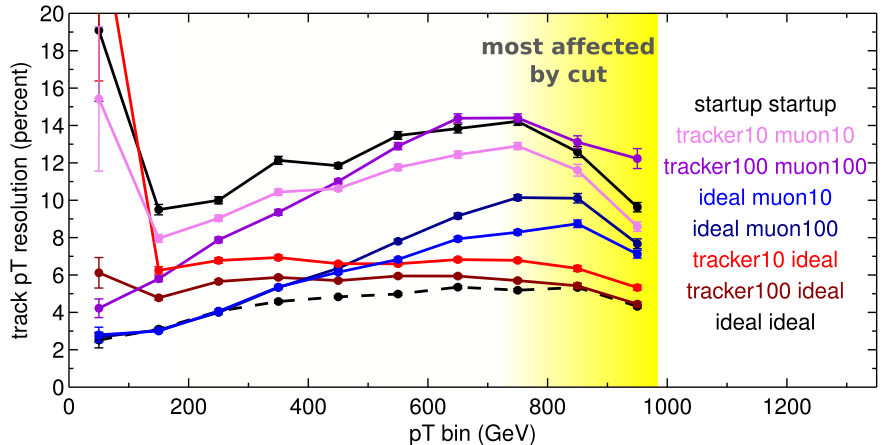
\includegraphics[width=\linewidth]{bypt_widths.png}
\end{frame}

\begin{frame}
\frametitle{Conclusions}
\begin{itemize}\setlength{\itemsep}{0.25 cm}
\item Plot-making apparatus is in place, reconstruction takes 4~hours (plus resubmissions)

\item Results independent of $Z'_{SSM}$ versus $Z'_\psi$ (good)

\item Some things I should look into: $\eta$ distributions, effect on
charge misassignment, relative importance of wheel/disk misalignments
and chamber misalignments

\item Comparison with toy misalignment?

\begin{itemize}\setlength{\itemsep}{0.2 cm}
\item reconstruction: 

\vspace{0.2 cm}
\begin{minipage}{0.8\linewidth}
\scriptsize \tt
include "Configuration/StandardSequences/data/FakeConditions.cff" \\
include "Configuration/StandardSequences/data/Reconstruction.cff" \\
\mbox{path p = \{ckftracks, muontracking, muons, MyAnalyzer\}} \\
\end{minipage}

with tracker and muon geometry from Frontier database

\vspace{0.1 cm}
\item MC-matching: closest in $\phi$ for $p_T > 20$~GeV globalMuons
\end{itemize}
\end{itemize}
\label{numpages}
\end{frame}

\end{document}
